\section{经验}
\label{sec:experience}

本节描述我们部署和运维 \sysname 的经验。

\parabf{部署经验。} \sysname 已部署在我们的生产环境中，并负责公司内部大多数大规模 MoE 训练任务。它支持训练拥有万亿参数的模型，支持单个训练作业扩展到超过 10,000 张 GPU，且单个训练任务可运行数月。通过结合前述技术，\sysname 在不损害模型性能的情况下，最小化 MoE 训练中的空闲通信时间并优化内存使用，最终在大规模 MoE 训练中节省数百万 GPU 小时。
图~\ref{fig:experience:llm-loss} 展示了一个真实生产作业中的模型收敛情况。该作业训练一个专有 MoE 模型，总参数量为 200B，每个 token 激活 20B 参数。该作业使用超过 10,000 张 GPU，持续数月。loss 在稳定训练过程中持续收敛。

\parabf{FP8 训练。} 为保持 FP8 训练的收敛稳定性，我们做了大量工作。例如，我们观察到 SwiGLU 算子会显著扩大数值范围。为解决该问题，我们用精度更高的按 token 量化（$1 \times h$）替代按 tensor 量化。此外，由于 SwiGLU 与 gating weight 相乘会进一步放大动态数值范围，我们将 gating weight 乘法后移到 FC2 输出之后，从而减少量化误差。

除了确保训练收敛，我们还引入了额外工程优化。现有 FP8 训练实现~\cite{transformer-engine, liang2024torchtitan} 以 BF16 存储模型参数，因此在 GEMM 计算前需要频繁转换到 FP8，增加了类型转换和转置开销。为解决该问题，我们使用多精度优化器，直接以 FP8 存储模型参数，同时将主参数保留为 FP32，并为不同数据类型使用独立 buffer。这降低了内存消耗，并将数据并行中的参数 all-gather 通信减半。

\parabf{扩展规模。} 在训练 MoE 模型时，一个有趣的工程问题是：能否在不增加计算负载的情况下，通过增加模型参数无限扩展训练规模？在张量并行中，这种方法并不实际，因为扩大模型需要更高 TP degree 来容纳额外参数。虽然增加 TP 会减少每张 GPU 上的计算，但如 式~\ref{eq:1} 和 \ref{eq:4} 所示，通信开销保持不变，导致通信时间逐渐变长并降低训练效率。换言之，TP 存在固有可扩展性限制，并且常依赖高速节点内链路来缓解通信延迟。

\begin{figure}[t!]
    \centering
    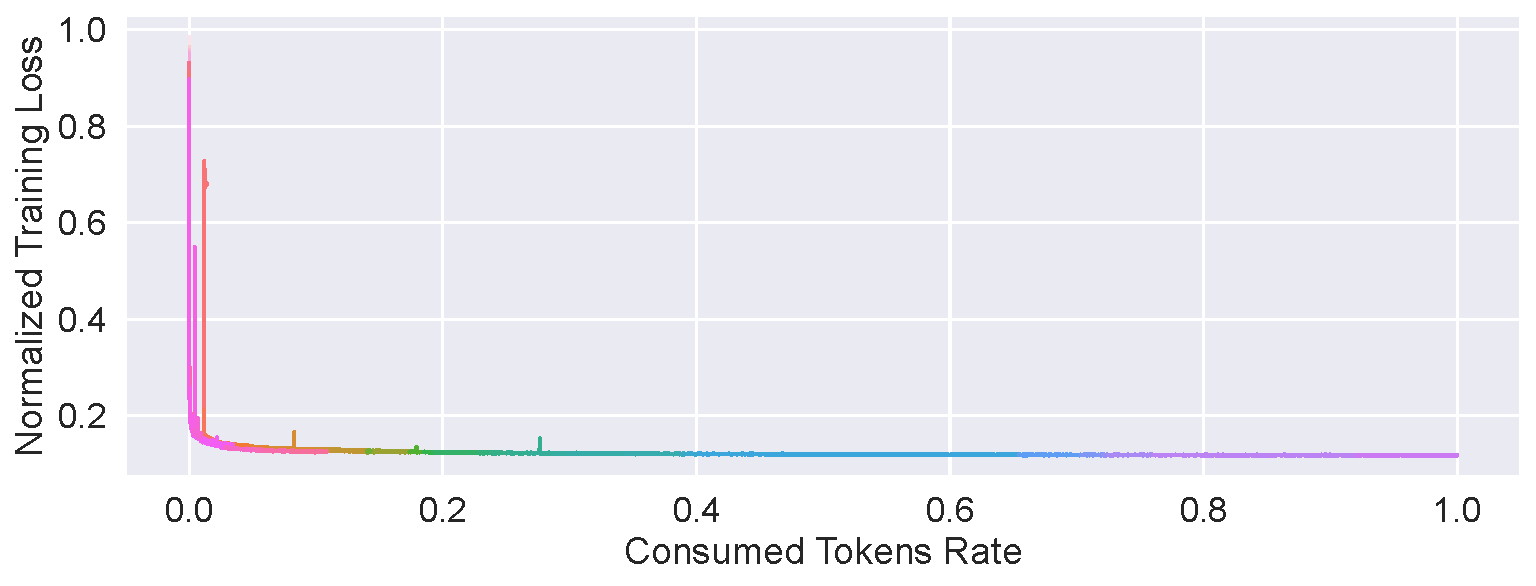
\includegraphics[width=\linewidth]{figures/llm-loss.pdf}
    \vspace{-0.2in}
    \caption{一个真实生产作业的归一化训练 loss 曲线。该作业在超过 10,000 张 GPU 上运行数月，在数万亿 token 上训练一个每次激活 20B 参数、总参数量 200B 的 MoE 模型。不同颜色表示训练重启。}
    \vspace{-0.1in}
    \label{fig:experience:llm-loss}
\end{figure}

相比之下，当使用 SP 和 EP 扩展训练时，如 式~\ref{eq:2} 和 \ref{eq:3} 所示，通信量会随着并行规模 $n$ 增大而下降。这意味着从理论上看，该并行策略可以扩展到显著更大的规模。然而，在实际层次化基础设施中，一个关键挑战随之出现：当扩展超出 NVLink 域、带宽下降到 RDMA 水平时，该方法能否保持训练效率？

形式化地，对于包含 MoE 机制的 SwiGLU 结构，计算时间与通信时间的比值 $R$ 定义为：
\begin{align}
    \text{comm\_time} & = \frac{2k \times bsh(n-1)/n /n}{bandwidth}, \\
    \text{comp\_time} & = \frac{3k \times bsh \times h_{ffn}/n}{peak}.
\end{align}
\begin{align}
    \hspace{-3cm} R &= \frac{\text{comp\_time}}{\text{comm\_time}} \\
    &= 3/2\times h_{ffn}\times \frac{bandwidth}{peak} \times n/(n-1) \\
    & \approx  3/2 \times h_{ffn} \times \frac{bandwidth}{peak}
\end{align}
为了维持训练效率，FFN 的计算时间必须超过通信时间，以确保通信开销能够被有效重叠。因此，我们的目标是保持 $R > 1$，这带来两个关键洞察：
\begin{itemize}[leftmargin=*]
    \item $R$ 的值与专家数量、top-$k$、隐藏维度、并行规模或输入大小无关，因此算法参数选择具有灵活性。
    \item $R$ 只由专家的中间维度、计算峰值和通信带宽决定。因此，在固定硬件上，只要专家维度足够大，从工程角度看，MoE 模型就可以在保持训练效率的同时继续扩展。
\end{itemize}

\parabf{整体化与自动化。} 我们在算子间通信-计算重叠上投入了大量工程工作，包括确定算子执行顺序、通信与计算的并发方式，以及通信的 SM 分配。这些人工干预帮助我们更深入理解训练动态，并支持有针对性的优化。随着训练推进和经验积累，我们希望在搜索空间内自动化算子调度，以细粒度优化训练过程并达到最优性能。自动优化留作未来工作。

\parabf{MoE 与稠密模型训练。} \revision{在持续优化 MoE 模型训练的过程中，我们识别出它与稠密模型训练之间的几个关键差异。在稠密 Transformer 层中，优化工作集中在自注意力和 GEMM 上。前者通常由 FlashAttention~\cite{dao2022flashattention} 等技术加速，而后者作为稠密计算，一般可以在 GPU 并行处理单元上达到较高利用率。相比之下，如 图~\ref{fig:eval:different_gpus}a 所示，注意力和 GroupedGEMM 的总运行时间只占一层执行时间的大约三分之一。其余时间由通信和其他算子消耗。尽管 \sysname 有效处理了通信开销，我们观察到 MoE 模型中的计算算子本身比稠密模型中的对应算子更复杂，也会引入性能下降。具体而言，它们是 straggler 的主要来源，原因有三点：}

\revision{第一，每个专家的中间维度小于稠密模型中的 FFN 层。为了高效并发处理多个专家的计算，GroupedGEMM 使用单个 CUDA kernel 执行大量小矩阵乘法。该 kernel 的资源使用，包括 shared memory、L1 cache 和线程数量，会通过 \texttt{cuFuncSetAttribute} 进行细粒度控制。然而，这种细粒度控制可能引入同步延迟。第二，由于路由到每个专家的 token 数量不均衡，GroupedGEMM 的输入和输出是动态形状张量。这些张量的频繁分配和释放会加剧 GPU 内存碎片。第三，MoE gating 机制涉及大量小算子，用于计算路由分数、通信路由决策等任务。CPU 性能抖动可能延迟这些 kernel 的启动，以至于启动延迟超过它们在 GPU 上的实际执行时间，从而产生流水线气泡。}

% \subsection{stability, trouble-shooting}

% \section{Candidate Topics Below}

% \subsection{Performance Analyze Platform}

% \subsection{Straggler Detection}

% \subsection{Fast Recovery}

% \subsection{Low precesion training}
